\documentclass{article}
\usepackage[brazil]{babel}
\usepackage[letterpaper,top=2cm,bottom=2cm,left=3cm,right=3cm,marginparwidth=1.75cm]{geometry}

\usepackage{amsmath}
\usepackage{graphicx}
\usepackage[colorlinks=true, allcolors=blue]{hyperref}

\title{Lista Especial de Problemas 11}
\author{Jeferson Almir}
\date{}

% 32

\begin{document}
\maketitle

\begin{enumerate}
    \item É possível particionar um quadrado em nove quadrados,
    com cinco deles de um tamanho,
    três com outro tamanho,
    e um de um terceiro tamanho?
    
    \item De um tabuleiro $9\times 9$,
    todas as 16 casas em que ambos os números da linha e coluna eram pares foram removidos.
    O tabuleiro com furos foi particionado em pedaços retangulares.
    Qual é a quantidade mínima de pedaços quadrados?
    
    \item A figura do diagrama a seguir pode ser cortada seguindo os pontilhados até restarem apenas quadrados,
    que não necessariamente são do mesmo tamanho.
    Qual é a quantidade mínima de quadrados que vai restar?
    
	\begin{center}
		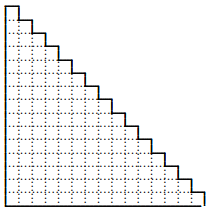
\includegraphics[scale=1]{img/img_11_01}
	\end{center}
    
    \item Num tabuleiro $10\times 10$,
    as 25 casas no subtabuleiro $5\times 5$ do canto superior esquerdo
    são pretas enquanto as restantes são brancas.
    O tabuleiro é dividido numa certa quantidade peças conexas
    de vários formatos e tamanhos
    de tal forma que a quantidade de casas brancas em cada peça é o triplo de casas pretas nessa peça.
    Qual é a quantidade máxima de peças?
    
    \item \begin{enumerate}
    \item Existe algum polígono não-convexo
    que pode ser particionado em duas partes conguentes por um segmento de reta
    que corta um lado do polígono original na metade,
    e outro lado na razão $1:2$?
    
    \item Tal polígono pode ser convexo?
    \end{enumerate}
    
    \item Existe algum hexágono que pode ser particionado
    em quatro triângulo congruentes por um único corte retilíneo?
    
    \item É possível particionar um polígono
    em quatro triângulos isósceles,
    sem haver dois deles congruentes,
    se o polígono é:
    
    \begin{enumerate}
    \item um quadrado?
    
    \item um triângulo equilátero?
    \end{enumerate}
    
    \item Karlos e Lédio estão dividindo um bolo quadrado.
    Karlos escolhe um ponto $P$ do bolo
    que não está sobre a borda.
    Lédio faz um corte reto de $P$ até a borda do bolo,
    na direção que quiser.
    Então, Karlos faz um corte reto de $P$ até a borda,
    de forma perpendicular ao primeiro corte.
    Lédio fica com o menor dos dois pedaços resultantes.
    É possível para Karlos prevenir Lédio de pegar ao menos um quarto do bolo?
    
    \item É possível particionar um cubo em dois pedaços
    que podem ser reunidos num poliedro convexo
    com apenas faces triangulares e hexagonais?
\end{enumerate}

\end{document}